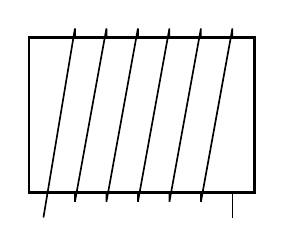
\begin{tikzpicture}[transform shape]
	% Paths, nodes and wires:
	\node[shape=rectangle, draw, line width=1pt, minimum width=2.865cm, minimum height=1.965cm] at (2.85, 1.8){};
	\draw[line width=0.6pt] (4, 0.496) -| (4, 0.796);
	\draw[line width=0.6pt] (1.6, 0.5) -- (2, 2.9) -- (2, 2.8);
	\draw[line width=0.6pt] (2, 0.8) -- (2, 0.7) -- (2.4, 2.9) -- (2.4, 2.8);
	\draw[line width=0.6pt] (2.4, 0.8) -- (2.4, 0.7) -- (2.8, 2.9) -- (2.8, 2.8);
	\draw[line width=0.6pt] (2.8, 0.8) -- (2.8, 0.7) -- (3.2, 2.9) -- (3.2, 2.8);
	\draw[line width=0.6pt] (3.2, 0.8) -- (3.2, 0.7) -- (3.6, 2.9) -- (3.6, 2.8);
	\draw[line width=0.6pt] (3.6, 0.8) -- (3.6, 0.7) -- (4, 2.9) -- (4, 2.8);
\end{tikzpicture}